% 固定源第16题图：原文“三棱锥”与六顶点图的矛盾保留待核。
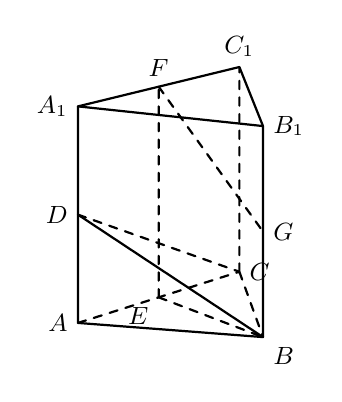
\begin{tikzpicture}[line cap=round,line join=round,thick,
  every node/.style={font=\small}]
  % Approximate oblique projection traced from the printed source figure.
  \coordinate (A) at (0,0);
  \coordinate (B) at (2.35,-.18);
  \coordinate (C) at (2.05,.65);
  \coordinate (A1) at (0,2.75);
  \coordinate (B1) at (2.35,2.5);
  \coordinate (C1) at (2.05,3.25);
  \coordinate (D) at (0,1.375);
  \coordinate (E) at (1.025,.325);
  \coordinate (F) at (1.025,3.0);
  \coordinate (G) at (2.35,1.16);
  % Outer edges and visible/hidden corresponding edges.
  \draw (A)--(A1) (A1)--(B1) (B1)--(B) (B)--(A);
  \draw (A1)--(C1) (C1)--(B1);
  \draw[dashed] (A)--(C) (C)--(B) (C)--(C1);
  % Internal construction segments shown in the original.
  \draw[dashed] (D)--(C) (E)--(B) (E)--(F);
  \draw[dashed] (F)--(G);
  \draw (D)--(B);
  % Point labels.
  \node[left] at (A) {$A$};
  \node[below right] at (B) {$B$};
  \node[right] at (C) {$C$};
  \node[left] at (A1) {$A_1$};
  \node[right] at (B1) {$B_1$};
  \node[above] at (C1) {$C_1$};
  \node[left] at (D) {$D$};
  \node[below left] at (E) {$E$};
  \node[above] at (F) {$F$};
  \node[right] at (G) {$G$};
\end{tikzpicture}
